%% TODO: aspect ratio
\documentclass[aspectratio=169,dvipsnames]{beamer}

\usepackage{amssymb,amsmath,amsthm,latexsym}
\usepackage{url,hyperref}
\usepackage{nccmath}            % fleqn environment
\usepackage{mathpartir}         % \mathpar, \infer
\usepackage{booktabs}           % \midrule
\usepackage{colonequals}
\usepackage{tikz,tikz-cd}       % Hasse & commutative diagrams.
\usepackage{accents}            % \underaccent

%% font fiddling
\usefonttheme{professionalfonts}
\renewcommand{\familydefault}{\rmdefault}
%\usepackage[scaled=0.9543]{XCharter}
\usepackage[semibold,scaled=0.9663]{sourceserifpro}
\usepackage[semibold,scaled=0.9663]{sourcesanspro}
%\usepackage[osf,scaled=1.0155]{AlegreyaSans}
\usepackage[scaled=1.00438,varqu,var0]{inconsolata}
\usepackage{eulervm}
\usepackage[bb=boondox]{mathalfa} % or bb=ams
\usepackage[T1]{fontenc}

%% TODO: more tracking for charter.
\usepackage[tracking,letterspace=20]{microtype}
\frenchspacing

\def\arraystretch{1.1}


%% ===== COMMANDS =====
\newcommand\strong\textbf

\newcommand\N{\mathbb{N}}
\newcommand\x\times
\newcommand\G\Gamma
\newcommand\D\Delta
\newcommand\fn{\ensuremath{\lambda}}
\newcommand\isa{\mathrel{\,\ratio\,}}

\newcommand{\setfor}[2]{\{{#1} \mathrel{|} {#2}\}}

\newcommand\kw[1]{\ensuremath{\textbf{#1}}}
\newcommand\n\mathit
\newcommand\tpname\mathrm
\newcommand\tset{\tpname{Set}~}
\newcommand\zero{\ensuremath{\mathbf{0}}}

\newcommand\fix{\n{fix}}
\newcommand\semifix{\n{semifix}}

\newcommand\naive{na\"ive}
\newcommand\Naive{Na\"ive}

\let\oldcup\cup\renewcommand\cup{\mathrel{\oldcup}}

\newcommand\hilite{\color{Rhodamine}}
\newcommand\hi[1]{{\hilite#1}}
%\newcommand\hilitetime{\color{Orange}}\newcommand\hiti[1]{{\hilitetime#1}}


\title{Semi\naive\ Evaluation for a Higher-Order Language}
\author{Michael Arntzenius}
\institute{University of Birmingham}
\date{POPL 2020}
\begin{document}
  \LARGE

  \begin{frame}
    \begin{fleqn}
      \[\begin{array}{l}
      \n{edge}, \n{path} \isa \tset (\N \x \N)
      \\
      \alt<1>{
        \hi{\n{path}} = \n{edge} \cup
        \setfor{(x,z)}{(x,y) \in \n{edge}, (y,z) \in \hi{\n{path}}}
      }{
        \n{step} \; {\only<2>{\hilite}s} = \n{edge} \cup
        \setfor{(x,z)}{(x,y) \in \n{edge}, (y,z) \in {\only<2>{\hilite}s}}
      }
      \\\pause
      \alt<3->{
        \n{path}_{\hi 0} = \emptyset
      }{\n{path} = \n{step} \; \n{path}}
      \\\pause
      \n{path}_{\hi{i+1}} = \n{step} \, \n{path}_{\hi i}
      \end{array}\]
    \end{fleqn}

    \vspace{1ex}
    \hspace{4pt}\Large(and wait until $\n{path}_i = \n{path}_{i+1}$)
  \end{frame}


  \begin{frame}
    \strong{Bottom-up fixed points} of \strong{monotone maps}:
    \vspace{1ex}

    \begin{itemize}\setlength\itemsep{1ex}
    \item Graph algorithms (eg.~shortest paths)
    \item Parsing (regexes, CFGs)
    \item Static analysis (abstract interpretation)
    \item \emph{Datalog!} {\normalsize\sffamily(if it's a map on finite sets)}
    \end{itemize}
  \end{frame}

  \begin{frame}
    Datalog is a \emph{first-order} logic language.
    \vspace{3ex}

    \pause
    \strong{Datafun}\textsuperscript{\sffamily\scshape[icfp 2016]}
    is a simply-typed \fn-calculus with:\vspace{1ex}
    \begin{itemize}\setlength\itemsep{1ex}
    \item a finite set datatype \& set comprehensions
    \item bottom-up monotone fixed points
    \item a type system that tracks monotonicity
    %% \item where types are posets, \\
    %%   and monotonicity is tracked in the type system
    \end{itemize}
    \vspace{1em}
  \end{frame}


  \begin{frame}
    \begin{mathpar}
      \begin{array}{l}
        \n{step} \; s = \n{edge} \cup
        \setfor{(x,z)}{(x,y) \in \n{edge}, (y,z) \in s}
        \\
        \n{path}_i = \n{step}^i \;\emptyset =
        \text{paths of length $\le i$}
      \end{array}
      \\\pause
      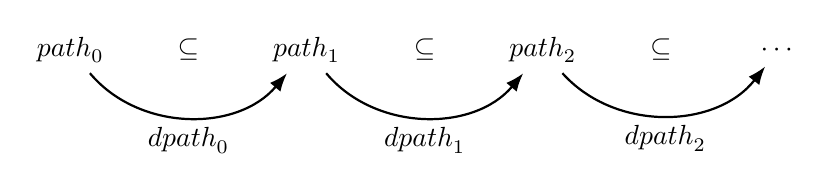
\begin{tikzpicture}[thick,baseline=(current bounding box.center), scale=1.5]
        \node (a) at (0, 0) {$\n{path}_0$};
        \node (ab) at (1, 0) {$\subseteq$};
        \node (b) at (2, 0) {$\n{path}_1$};
        \node (bc) at (3, 0) {$\subseteq$};
        \node (c) at (4, 0) {$\n{path}_2$};
        \node (cd) at (5, 0) {$\subseteq$};
        \node (d) at (6, 0) {$\cdots$};
        \path[-Latex, bend right=50,below]
          (a) edge node {$\n{dpath}_0$} (b)
          (b) edge node {$\n{dpath}_1$} (c)
          (c) edge node {$\n{dpath}_2$} (d);
      \end{tikzpicture}
    \end{mathpar}
  \end{frame}

  \begin{frame}{}{}\centering\setlength\baselineskip{2em}

    {\scshape semi\naive\ evaluation}

    {means}

    {\bf computing the changes between iterations}

    {by}

    {\bf incrementalizing the step function}
  \end{frame}


  \begin{frame}{}{}
    \begin{fleqn}[1em]
    {\bfseries\boldmath Incremental \fn-calculus} \textsuperscript{\sffamily\scshape[pldi 2014]}

    \begin{align*}
      \makebox[1.2cm][r]{$\alt<2->{\n{step}}{f}$} &\isa \alt<2->{\tset A \to \tset A}{A \to B}\\
      \alt<2->{\n{step}}{f}' &\isa
      \alt<2->{
        \underaccent{\parbox[t][1.4cm]{1.5cm}{\uncover<3->{\centering\vspace{4pt}\small\sffamily paths of length $< i$}}
        }{\tset A}
        \to \only<3->{\underaccent{\parbox{2cm}{\centering\vspace{4pt}\small\sffamily paths of length $i$}%
        }}{\hi{\alt<3->{\tset A}{\D(\tset A)}}}
        \to \only<3->{\underaccent{\parbox{2cm}{\centering\vspace{4pt}\small\sffamily paths of length $i+1$}%
        }}{\hi{\alt<3->{\tset A}{\D(\tset A)}}}
      }{
        \underaccent{\parbox{1.3cm}{\centering\vspace{4pt}\small\textsf{input}}}{A}
        \to \underaccent{\parbox{1.3cm}{\centering\small\sffamily\vspace{4pt} change to input}}{\D A}
        \to \underaccent{\parbox[t][1.4cm]{1.3cm}{\centering\small\sffamily\vspace{4pt} resulting change in output}}{\D B}
      }
    \end{align*}

    \pause\pause\pause
    \begin{align*}
      \n{path}_0 &= \emptyset
      & \n{path}_{i+1} &= \n{path}_i \cup \n{dpath}_{i}\\
      \n{dpath}_0 &= \n{step} \;\emptyset
      & \n{dpath}_{i+1} &= \n{step}' \;\n{path}_i \;\n{dpath}_i
    \end{align*}

    \vspace{1ex} Let $\semifix\;(\n{step}, \n{step}') = \n{path}_i$ st.
    $\n{path}_i = \n{path}_{i+1}$.
    \end{fleqn}
    %% \begin{align*}
    %%   f &\isa A \to B\\
    %%   f' &\isa \underaccent{\parbox{1.3cm}{\centering\vspace{4pt}\small\textsf{input}}}{A}
    %%     \to \underaccent{\parbox{1.3cm}{\centering\small\sffamily\vspace{4pt} change to input}}{\hi{\D A}}
    %%     \to \underaccent{\parbox{1.3cm}{\centering\small\sffamily\vspace{4pt} resulting change in output}}{\hi{\D B}}
    %% \end{align*}
  \end{frame}

  %% \begin{frame}
  %%   \begin{fleqn}
  %%   \begin{align*}
  %%     \n{step} &\isa \tset A \to \tset A\\
  %%     \n{step}' &\isa
  %%     \underaccent{\parbox{1.3cm}{\centering\vspace{4pt}\small\sffamily previous paths}}{\tset A}
  %%     \to \underaccent{wub
  %%     }{\hi{\alt<2->{\tset A}{\D(\tset A)}}}
  %%     \to \hi{\alt<2->{\tset A}{\D(\tset A)}}
  %%   \end{align*}
  %%   \end{fleqn}
  %% \end{frame}


  \begin{frame}\Large
    %\begin{center}\scshape the core idea\end{center}

    On any expression $e$, we define two
    mutually recursive static transformations:\vspace{1ex}
    \begin{itemize}\setlength\itemsep{1ex}
    \item \hi{$\phi e$} computes $e$ faster by replacing $\fix$ by $\semifix$.

    \item \hi{$\delta e$} incrementalizes $\phi e$ just enough to find the
      derivatives $\semifix$ needs.
    \end{itemize}
    \vspace{1ex}

    We:\vspace{1ex}
    \begin{itemize}\setlength\itemsep{1ex}
    \item Prove these correct using a logical relation.
    \item Implement them \& test their asymptotic performance.
    \end{itemize}
  \end{frame}
\end{document}


